% Options for packages loaded elsewhere
\PassOptionsToPackage{unicode}{hyperref}
\PassOptionsToPackage{hyphens}{url}
\PassOptionsToPackage{dvipsnames,svgnames,x11names}{xcolor}
%
\documentclass[
]{article}
\usepackage{amsmath,amssymb}
\usepackage{iftex}
\ifPDFTeX
  \usepackage[T1]{fontenc}
  \usepackage[utf8]{inputenc}
  \usepackage{textcomp} % provide euro and other symbols
\else % if luatex or xetex
  \usepackage{unicode-math} % this also loads fontspec
  \defaultfontfeatures{Scale=MatchLowercase}
  \defaultfontfeatures[\rmfamily]{Ligatures=TeX,Scale=1}
\fi
\usepackage{lmodern}
\ifPDFTeX\else
  % xetex/luatex font selection
\fi
% Use upquote if available, for straight quotes in verbatim environments
\IfFileExists{upquote.sty}{\usepackage{upquote}}{}
\IfFileExists{microtype.sty}{% use microtype if available
  \usepackage[]{microtype}
  \UseMicrotypeSet[protrusion]{basicmath} % disable protrusion for tt fonts
}{}
\makeatletter
\@ifundefined{KOMAClassName}{% if non-KOMA class
  \IfFileExists{parskip.sty}{%
    \usepackage{parskip}
  }{% else
    \setlength{\parindent}{0pt}
    \setlength{\parskip}{6pt plus 2pt minus 1pt}}
}{% if KOMA class
  \KOMAoptions{parskip=half}}
\makeatother
\usepackage{xcolor}
\usepackage[margin=1in]{geometry}
\usepackage{graphicx}
\makeatletter
\def\maxwidth{\ifdim\Gin@nat@width>\linewidth\linewidth\else\Gin@nat@width\fi}
\def\maxheight{\ifdim\Gin@nat@height>\textheight\textheight\else\Gin@nat@height\fi}
\makeatother
% Scale images if necessary, so that they will not overflow the page
% margins by default, and it is still possible to overwrite the defaults
% using explicit options in \includegraphics[width, height, ...]{}
\setkeys{Gin}{width=\maxwidth,height=\maxheight,keepaspectratio}
% Set default figure placement to htbp
\makeatletter
\def\fps@figure{htbp}
\makeatother
\setlength{\emergencystretch}{3em} % prevent overfull lines
\providecommand{\tightlist}{%
  \setlength{\itemsep}{0pt}\setlength{\parskip}{0pt}}
\setcounter{secnumdepth}{-\maxdimen} % remove section numbering
\ifLuaTeX
  \usepackage{selnolig}  % disable illegal ligatures
\fi
\usepackage[]{biblatex}
\addbibresource{ReferencesProject1.bib}
\IfFileExists{bookmark.sty}{\usepackage{bookmark}}{\usepackage{hyperref}}
\IfFileExists{xurl.sty}{\usepackage{xurl}}{} % add URL line breaks if available
\urlstyle{same}
\hypersetup{
  colorlinks=true,
  linkcolor={Maroon},
  filecolor={Maroon},
  citecolor={Blue},
  urlcolor={blue},
  pdfcreator={LaTeX via pandoc}}

\author{}
\date{\vspace{-2.5em}}

\begin{document}

\section{Introduction}\label{introduction}

Portugal has been long celebrated for its wine production, from port
wine to \emph{vino verde} from the Minho province. To address growing
demand, the wine industry is interested in optimising its wine
production. As wine is a food product, most of its prized features are
taste and aroma, which are subjective measurements. Previous studies
have tried to categorise wine by quality through combining human taste
testers, physicochemical analysis and statistical methods in attempts to
introduce objectivity\textsuperscript{1}. In this project, we are most
concerned with which \textbf{particular variables} are essential for
considering wine quality. By knowing which variables should be
prioritised, this can motivate further study on optimising the wine
according to essential attributes and enforce more efficient production.

Therefore, this report aims to address the following questions:

\begin{enumerate}
\def\labelenumi{\arabic{enumi}.}
\tightlist
\item
  What are the main chemical differences between red and white wines?
\item
  Which variables are associated with wines of higher quality overall,
  and for red and white wine individually?
\item
  Are there any differences between mean acidity values of wine?
\item
  Are there any differences between mean sulfate/sulfur dioxide values
  of wine?
\end{enumerate}

The dataset utilized in this study is drawn from laboratory tests,
offering a detailed examination of the chemical composition of wines
from Portugal's Minho region. It includes an extensive array of
variables such as fixed acidity, volatile acidity, citric acid, residual
sugar, chlorides, free sulfur dioxide, total sulfur dioxide, density, pH
levels, sulphates, alcohol content, and a subjective quality rating on a
scale of 0 to 10, where 10 signifies the highest quality. Additionally,
a color indicator, acting as a dummy variable, distinguishes between red
and white wines.

The data underwent outlier checking, with a total size of 6497 entries.
To balance outlier removal without sacrificing too much data, a 5\%
threshold (325 entries) was set as the maximum limit for removal. An
Interquartile Range (IQR) check was applied, a common procedure
involving data less than Q1 - 1.5IQR or more than Q3 + 1.5IQR. However,
due to a significant loss of data, a stricter threshold of 2.5 was
chosen instead.

\subsection{PCA - Chemical differences between red and white
wines}\label{pca---chemical-differences-between-red-and-white-wines}

\begin{figure}
\centering

\includegraphics[width=0.5\textwidth,height=\textheight]{Scree_plot.png}
\caption{Scree plot of explained variance ratio for each principle
component}
\end{figure}

Looking at the scree plot, the elbow appears around n = 3 components, so
we will use this when proceeding with our PCA model. When considering
the key chemical differences between red and white wines, we need to
identify which features produce large loadings for our model. These
features will help maximise the lagrange multiplier, producing the
largest variance which is essential in differentiating the chemical
differences between red and white wines.

\begin{figure}
\centering
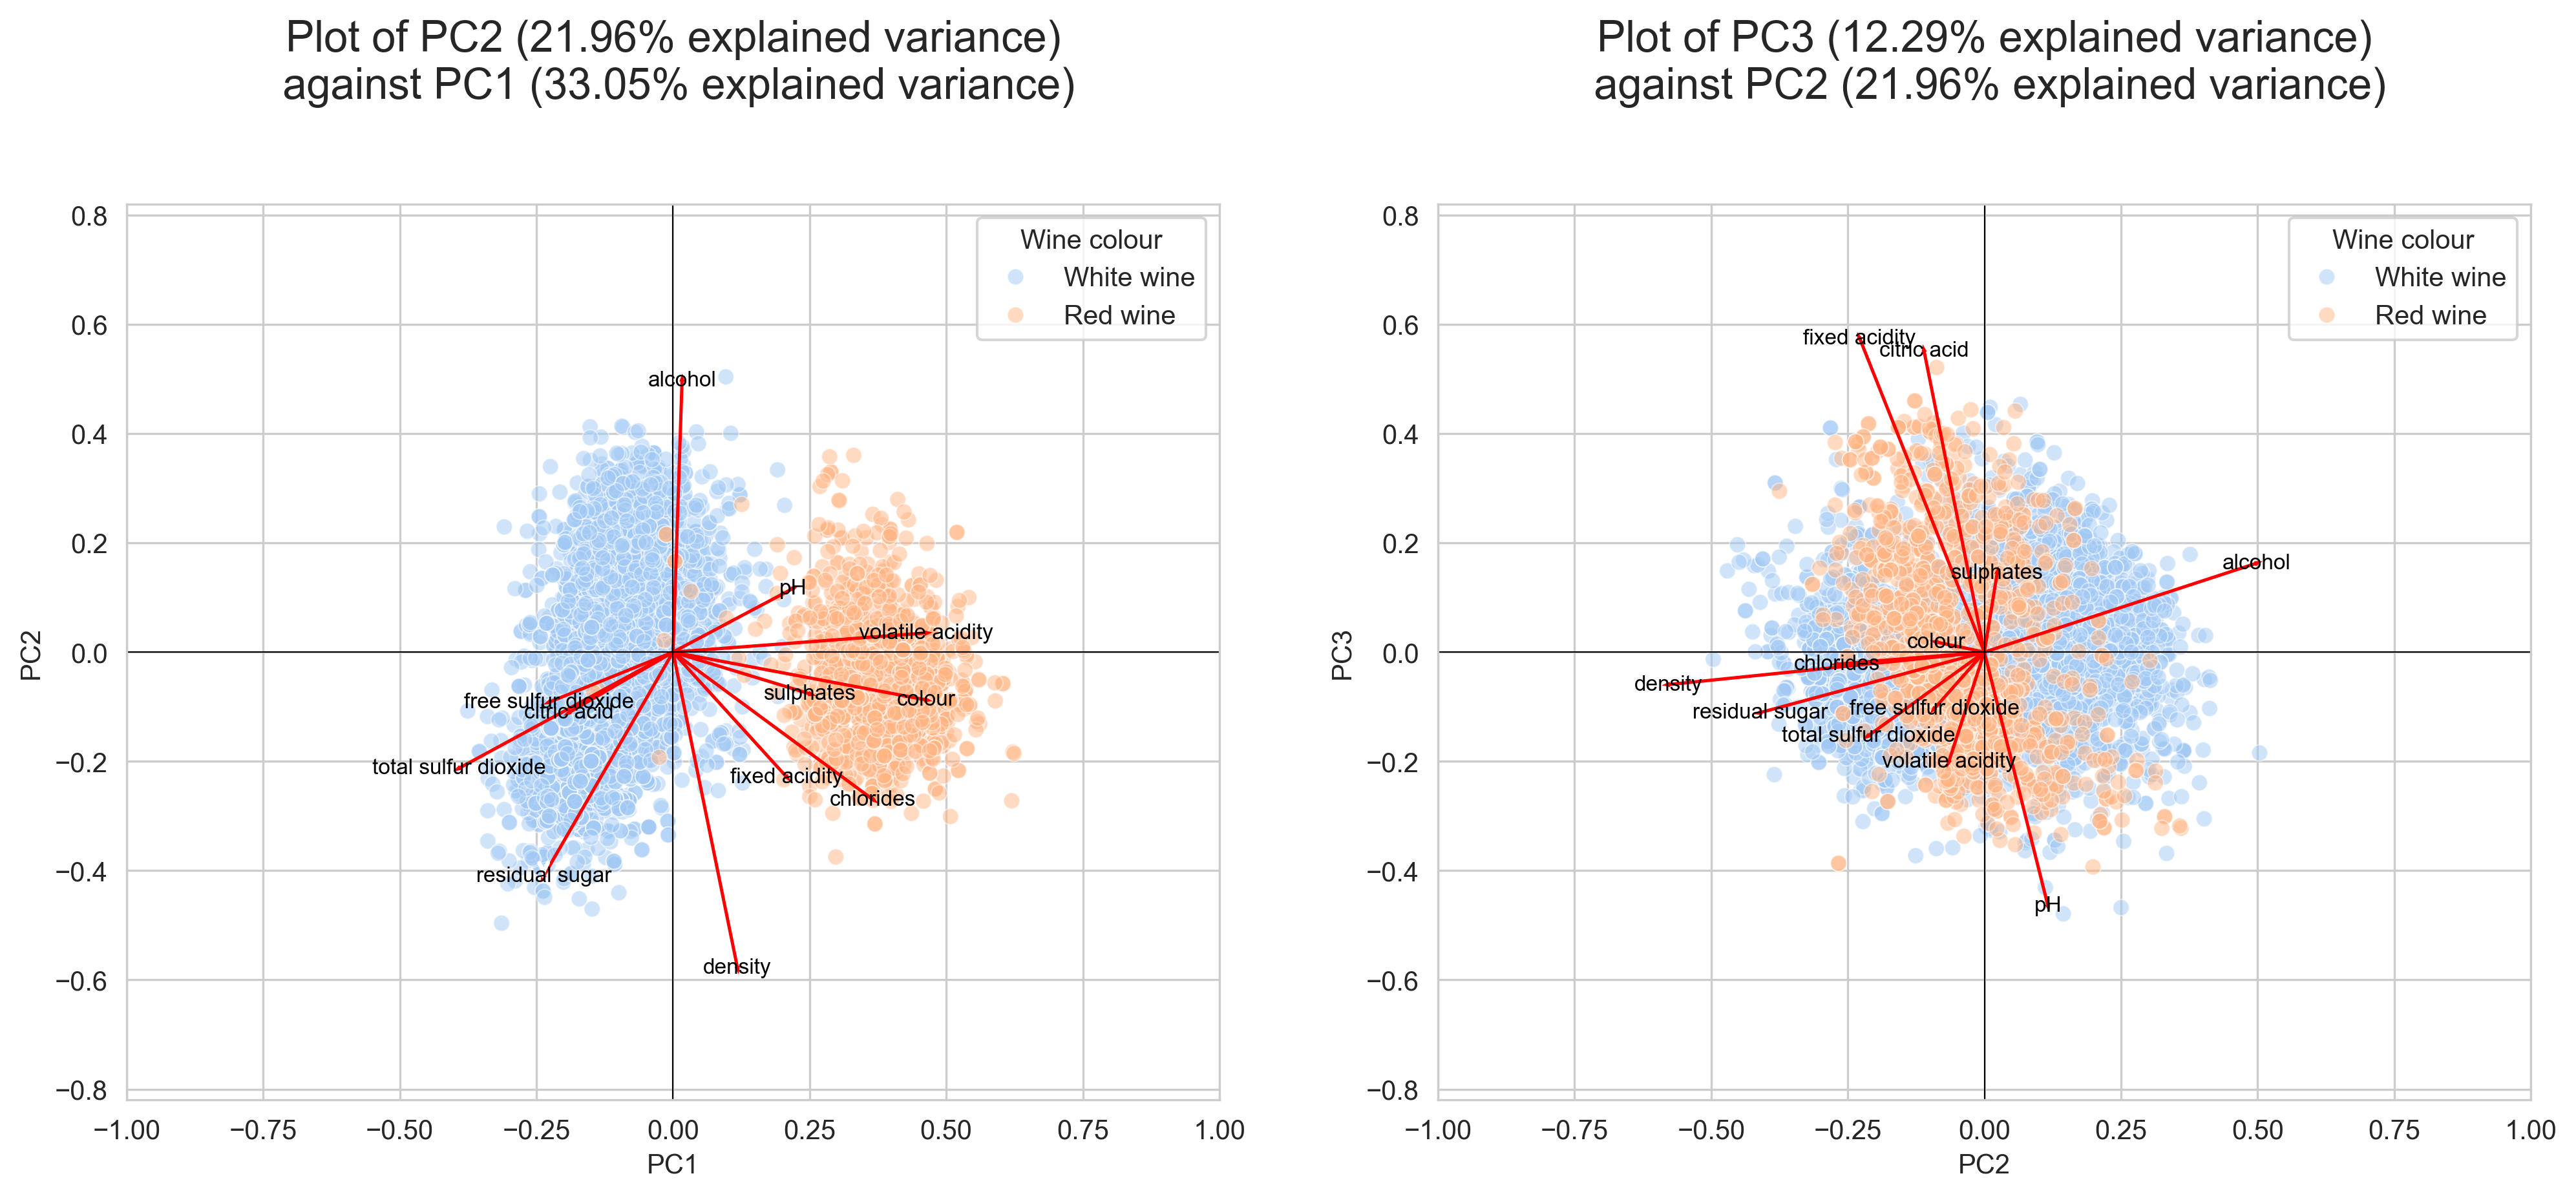
\includegraphics{biplots_combined_no_quality_new.png}
\caption{Bi-plots of loadings and scores for PC1 to PC3 of dataset but
no quality column}
\end{figure}

\subsubsection{PC1 component analysis}\label{pc1-component-analysis}

From the left biplot, we observe positive loadings for pH, volatile
acidity, sulfites (free sulfur dioxide, total sulfur dioxide), colour,
fixed acidity, density and chlorides. Notably, colour is coded as a
binary dummy variable, where 0 is white wine and 1 is red wine.
Therefore, \textbf{red wines will score higher on PC1 than white wines}.
We can use this to extrapolate any relationships between the colour
variable and other chemical metrics. All other factors being equal,
white wines with high volatile acidity and chlorides can score nearly as
high as red wines with low volatile acidity and chlorides. This suggests
that there is a positive correlation between a wine colour, volatile
acidity and chloride concentration, implying that \textbf{red wines tend
to have higher volatile acidity and chlorides than white wines}. The
increased fixed acidity concentration could be due to how red wines use
the seed and skin in addition to the pulp, which tend to contain more
tartaric acid whereas white wines only tend to use the pulp, thus
increasing the fixed acidity of red wines.\textsuperscript{2}

Paradoxically, wines with a higher pH (implies less acidic solution) and
acidic traits tend to score higher in PC1, but this can be explained as
these wines tend to have higher sulphates, which are basic and increase
the pH of the alcohol. This suggests that \textbf{red wines tend to have
a higher pH than white wines from the sulphate
content}.\textsuperscript{3}

Alcohol and density seem to have little difference between red and white
wines, indicating that alcohol and density are not key chemical
differentiators between and white wines.

For the left quadrants of the left plot, we can see negative loadings
for residual sugar, sulfites and citric acid. We have previously deduced
that positive loadings imply properties more associated with red wine,
hence higher values for the aforementioned properties are related to
white wines. In particular the data suggests that \textbf{white wines
tend to have higher levels of sulfites than red wines}. This is expected
as white wines are more susceptible to oxidation than red wines, so more
sulfur dioxide is used to act as an anti-microbal
agent\textsuperscript{3,4}.

\textbf{Conclusion: The data suggests that the main chemical differences
are red wines tend to contain more acids but have a higher pH than white
wines to balance out its acidity. In contrast, white wines tend to
contain sulfur dioxide than red wines to help prevent microbial growth.}

\subsection{PC2 and PC3 analysis}\label{pc2-and-pc3-analysis}

For completeness, we will check the right plot to check our conclusions
drawn from the previous section. For PC2 and PC3, for all things being
equal, the wine colour does not affect the PC2/PC3 scores, suggesting
that different wine characteristics as a whole will influence the score.
To score highly for PC2, wines need to have high alcohol concentrations
with low density, sulfites, chlorides and residual sugar. As sugar is
used by yeast to produce alcohol, this could account for wines that use
sweeter grape varieties, wines that score the highest include low
residual sugar but higher amounts fo alcohol. To score higher on PC3,
wines need to have low pH with high fixed acidity and citric acid. This
category could be a measure of extra components added to the wine to
enhance flavour and aroma, as citric acid is commonly added to introduce
freshness.\textsuperscript{5}

\subsection{PCA - Attributes present in wines of high
quality}\label{pca---attributes-present-in-wines-of-high-quality}

As the quality variable contains many categories, it makes it difficult
to visualise. Thus, the data was grouped into three categories, such
that \(x_{low_quality} \in [3, 4, 5]\), \(x_{medium_quality} \in [6]\)
and \(x_{high_quality} \in [7, 8, 9]\), then further divided by wine
colour. The PCA model in question does not use this dummy feature in its
fit, only the colour and quality instead.

\begin{figure}
\centering
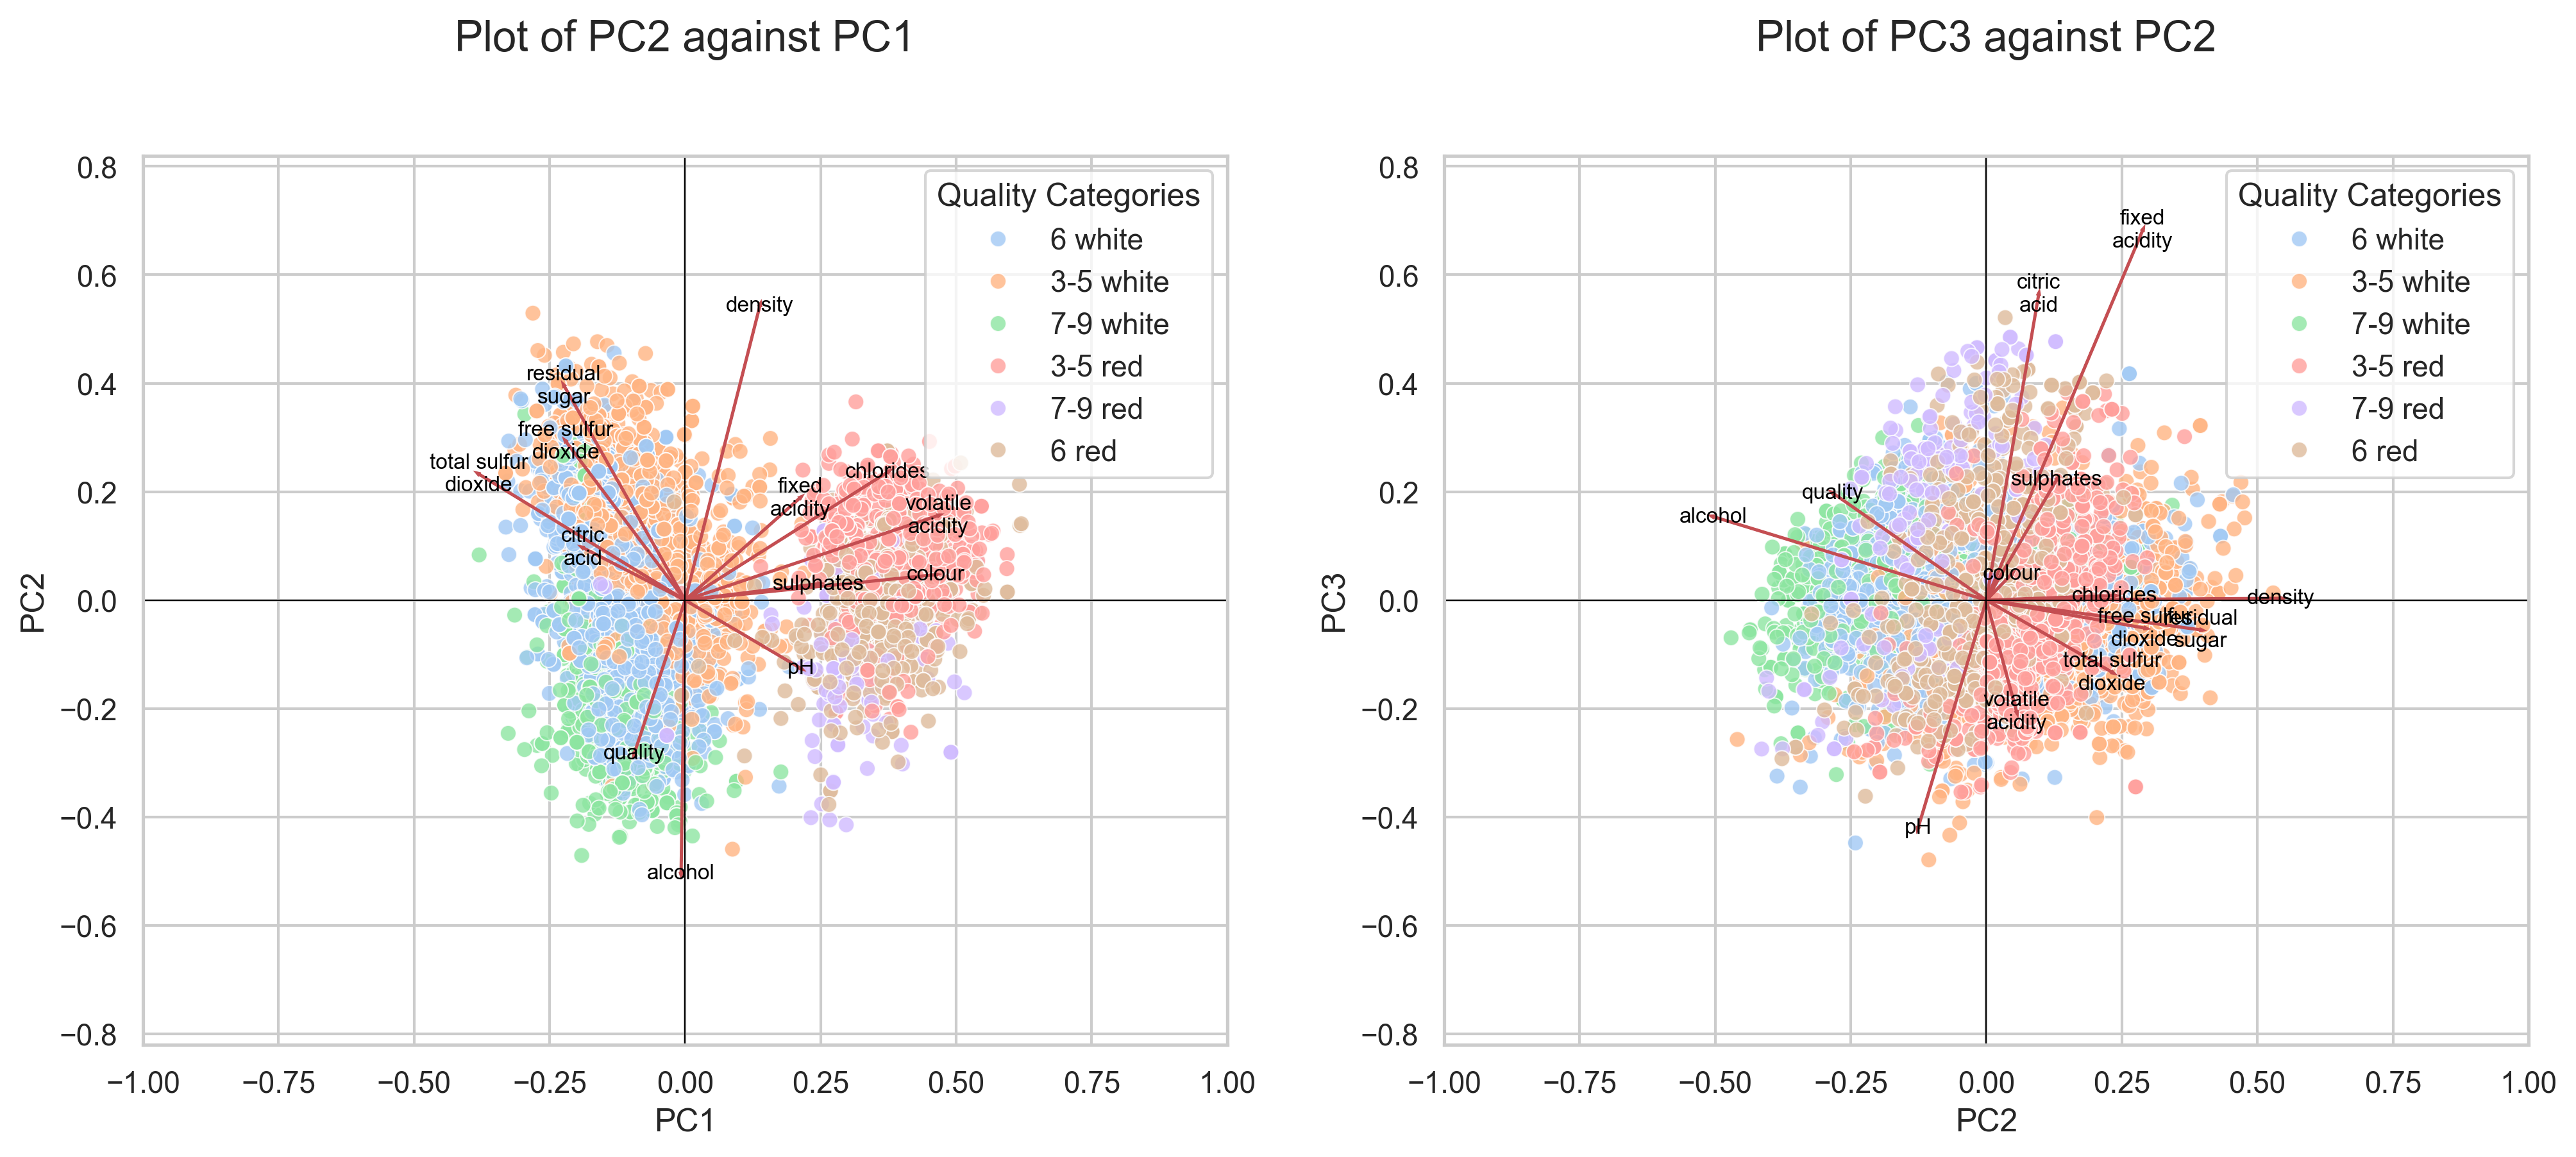
\includegraphics{wine_quality_pc2_vs_pc1_with_quality_new.png}
\caption{Bi-plots of loadings and scores for PC1 to PC3 of dataset with
quality column}
\end{figure}

\subsubsection{Analysis - alcohol}\label{analysis---alcohol}

When considering the left plot, we can see for higher quality wines
overall have negative PC2 scores but high quality red wine has a
positive PC1 score and high quality white wine has a negative PC1 score.
As the alcohol loading is close to zero for PC1 but large and negative
for PC2, this suggests that higher alcohol concentrations are more
likely to be present for wines of higher quality. Furthermore, as most
of datapoints for wine types are divided by PC1=0 line (whites on left,
reds on right), we can say this property \textbf{is not unique to red or
white wine, rather it applies to both of them}. This is further
supported by looking at the right plot, where most of the high quality
wines lie in the top left quadrant of the plot and the quality/alcohol
arrows point in the same direction.

\subsubsection{Analysis - volatile
acidity}\label{analysis---volatile-acidity}

Observing both plots we can see that greater volatile acidity is more
associated with lower quality wines as the arrow is in the same quadrant
as 3-5 red and 5 red points. In particular, it appears to be specific to
red wines as the volatile acidity is more associated with red wine as
seen in our previous analysis, therefore, \textbf{lower volatile acidity
is likely to be present in higher quality red wines}.

\subsubsection{Analysis - fixed acidity}\label{analysis---fixed-acidity}

Total sulfur dioxide has small positive PC1, PC2 scores but a large and
positive PC3 score. As more quality wines tend to lie on the bottom
quadrants (negative PC2 scores), we can deduce that higher quality wines
will tend to have lower fixed acidity than lower quality wines. This is
further supported by the right plot, where the fixed acidity loading is
in the right quadrants, which tends to be where most of the lower
quality wines are. Fixed acidity while more associated with red wine
from the plots, some lower quality white wine loadings are present in
the same quadrant (though not as much) suggesting \textbf{lower fixed
acidity is likely to be present in higher quality red wines and white
wines (to a lesser degree)}.

\subsection{Conclusion}\label{conclusion}

In summary, higher quality wines tend to have higher alcohol levels and
lower volatile/fixed acidities. When factoring in by wine type and their
chemical differences, it seems volatile acidity plays a key role in
determining not only wine type but its quality for red wines as well.
Therefore, further research should be concentrated on optimising fixed
acidity levels to produce high quality wines.

\section{Hotelling T square test}\label{hotelling-t-square-test}

So far, we have explored what particular features are present for wines
of good quality, as well as main chemical differences between red and
white wines. We highlighted that volatile and fixed acidity are
different for red and white wines, but we should verify this through a
statistical test. As our data is multivariate, we cannot perform a
standard two sample student t-test, but we can instead perform a \emph{A
hotelling \(T^2\) test}. For a 2 group case (red and white wine), we can
perform a MANOVA fit and obtain the Hotelling \(T^2\) statistic and the
F-value. Confidence intervals were calculated using a function I wrote
myself based on statistical theory. The hotelling T statistic is 1.66
and the F-value is 3292.11. See code for details.

\textbf{H0}: The mean volatile acidity, fixed acidity and pH are equal
for both red and white wines

There is very strong evidence (p\textless0.001) to reject the null
hypothesis that the mean volatile acidity, fixed acidity and pH are
equal for both red and white wines. It seems at least one of the acidity
means for red wine is different to white wine with averages of volatile
acidity 0.23 95\% simultaneous CI (-28.35, 27.85) g(acetic
acid)/dm\(^3\), fixed acidity 1.10 95\% simultaneous CI (-256.65,
253.73) g(tartaric acid)/dm\(^3\), pH 0.14 95\% simultaneous CI (-34.34,
34.09). As a follow-up analysis, we can produce boxplots to see which
particular acid metric is the most different.

\begin{figure}
\centering
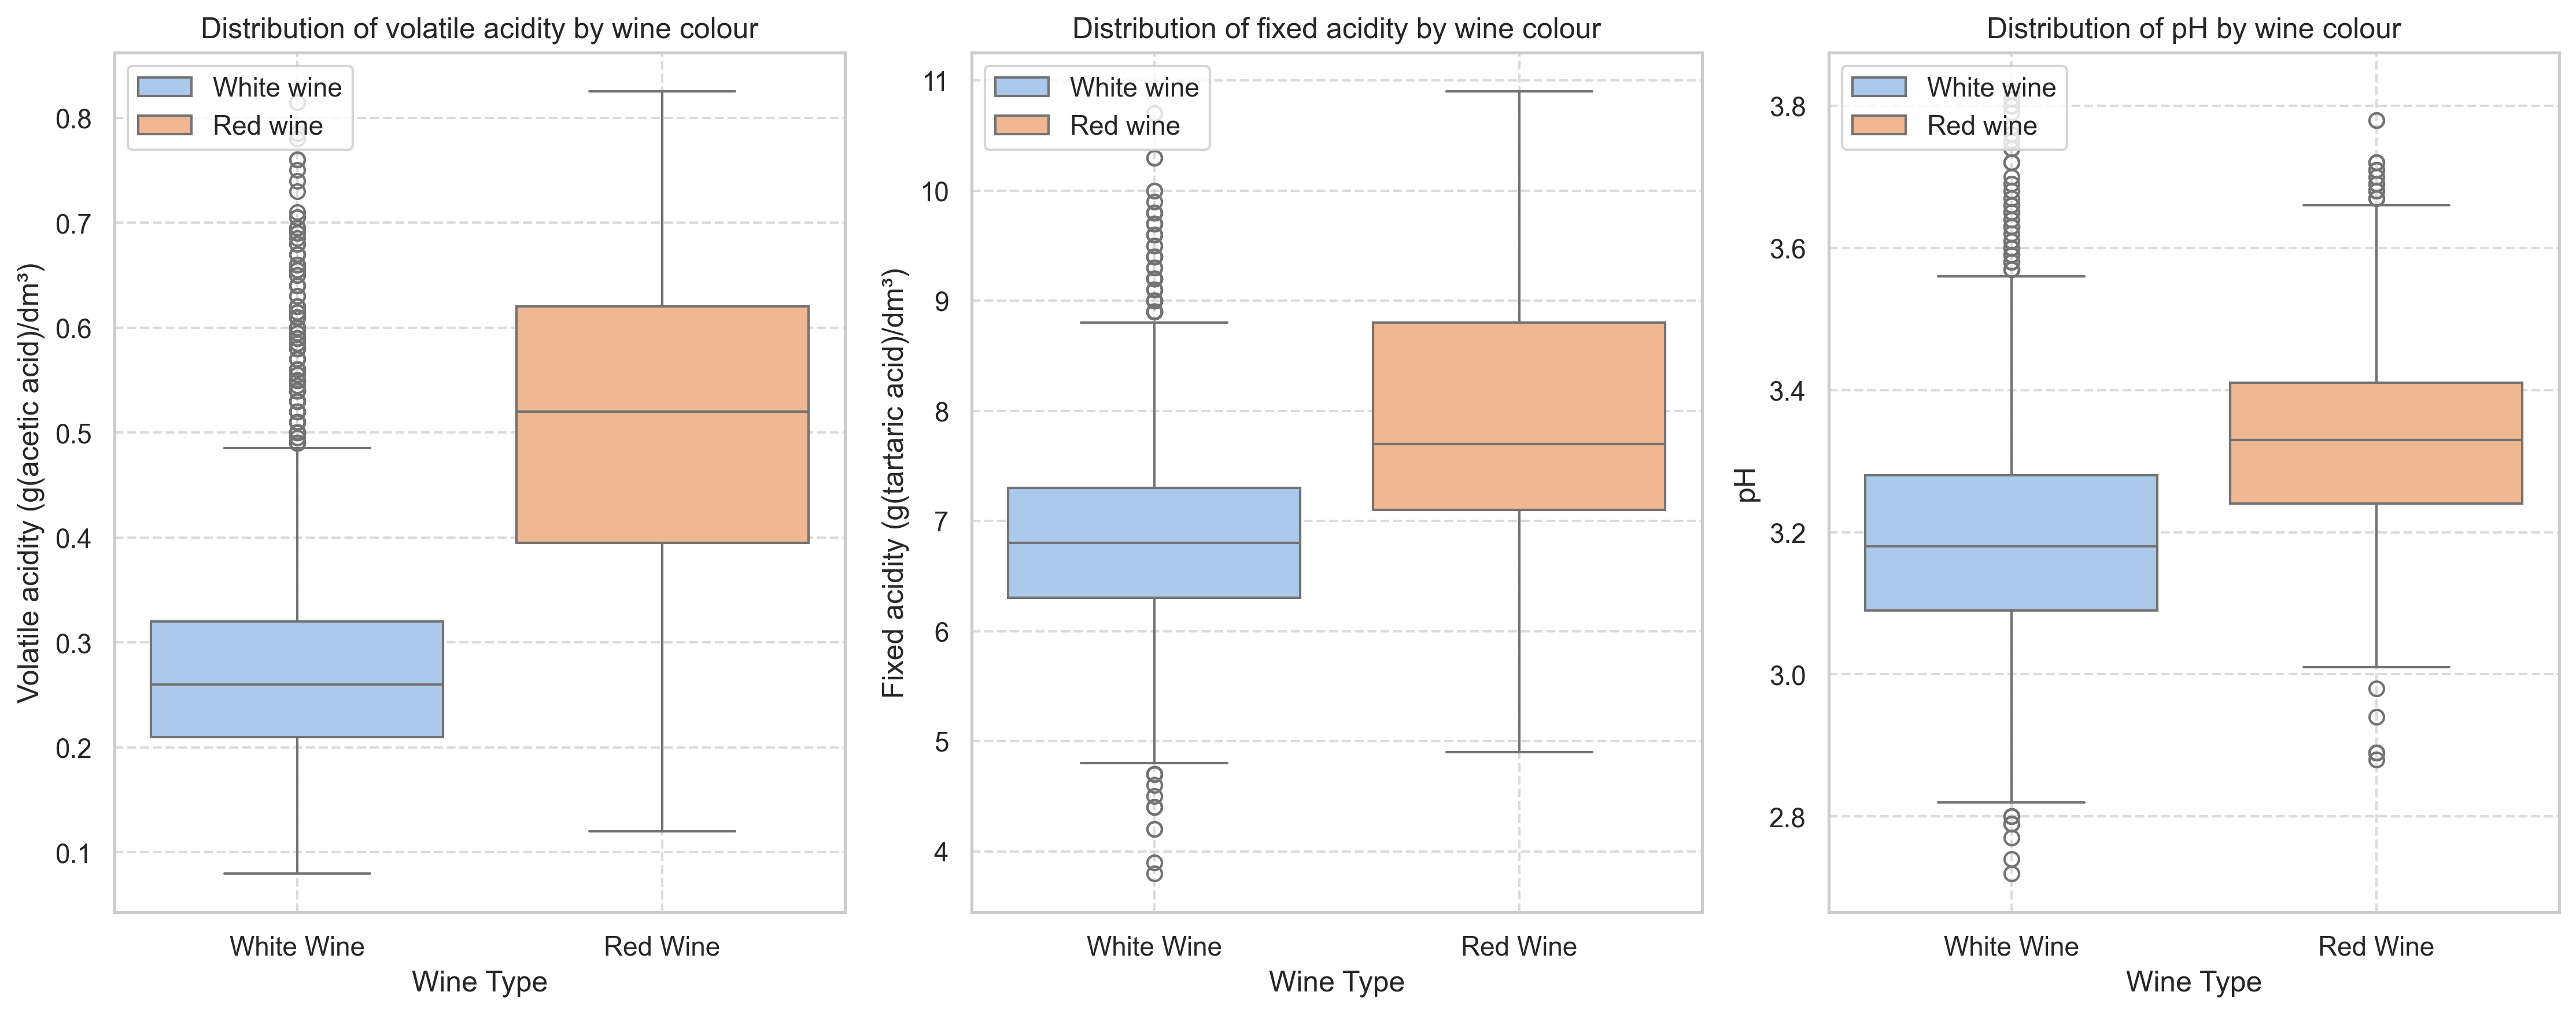
\includegraphics{box_plots_for_hotelling_two_sample.png}
\caption{Boxplot for post-hoc Hotelling T\textsuperscript{2} analysis}
\end{figure}

From the boxplots, it seems most of the red wine volatile acidity tends
to have higher mean values than white wine, which could explain why the
test result was statistically significant.

\subsection{Hotelling T test - 1
sample}\label{hotelling-t-test---1-sample}

Sulphates and sulfur dioxide have not been explored much in this report
compared to acidity, but they still play an important role to wine
quality as they affect wine aroma. The sample means of white wine for
free sulfur dioxide, total sulfur dioxide and sulphates were calculated
to be 34.92 mg/dm\(^3\), 137.80 mg/dm\(^3\) and 0.49 g(potassium
sulphate)/dm\(^3\) respectively. Statsmodels comes with a 1 sample
hotelling t test if you use test\_mvmean
\texttt{from\ statsmodels.stats.multivariate\ import\ test\_mvmean}
\href{https://www.statsmodels.org/dev/generated/statsmodels.stats.multivariate.test_mvmean.html}{as
shown here in their docs}. The F statistic is 3682.53 (2dp) and the
hotelling value is 11064.99 (2dp)

\textbf{H0}: The mean free sulfur dioxide, total sulfur dioxide and
sulphates for white mean are equal to the sample means for red wine

There is very strong evidence (p\textless0.001) to reject the null
hypothesis that the mean free sulfur dioxide, total sulfur dioxide and
sulphates are equal for both red and white wines. It seems at least one
of the sulfate means for red wine is different to white wine with
averages of free sulfur dioxide -18.61 95\% simultaneous CI (-1011.28,
1043.90) g/dm\(^3\), total sulfur dioxide -90.95 95\% simultaneous CI
(-3210.83, 3304.53) g/dm\(^3\), sulphates 0.14 95\% simultaneous CI
(-11.16, 12.43) g(potassium sulphate)/dm\(^3\). As a follow up analysis,
we can produce boxplots to see which particular sulphate metric is the
most different (Omitted due to space, but code available to generate
them). From the boxplots, it seems most of the red wine total sulfur
dioxide tends to have higher mean values than white wine, which could
explain why the test result was statistically significant.

\subsubsection{References}\label{references}

\begin{enumerate}
\def\labelenumi{\arabic{enumi}.}
\tightlist
\item
  CORTEZ, P., CERDEIRA, A. L., ALMEIDA, F., MATOS, T. \& REIS, J. 2009.
  Modeling wine preferences by data mining from physicochemical
  properties. Decis. Support Syst., 47, 547-553.
\item
  SOKAČ CVETNIĆ, T., GUNJEVIĆ, V., PUŠEK, A., JURINJAK TUSEK, A.,
  DUJMIĆ, F., BRNCIC, M., KOVAČEVIĆ GANIĆ, K., JAKOVLJEVIĆ, T., UHER,
  D., MITRIĆ, G. \& RADOJCIC REDOVNIKOVIC, I. 2022. Comparison of Drying
  Methods and Their Effect on the Stability of Graševina Grape Pomace
  Biologically Active Compounds. Foods, 11, 112.
\item
  PEZLEY, M. E. 2023. Production of free sulfur dioxide by wine yeasts.
\item
  NIOI, C., LISANTI, M. T., MEUNIER, F., MASSOT, A. \& MOINE, V. 2023.
  Yeast derivatives: a promising alternative for white wine oxidation
  prevention. IVES Technical Reviews, vine and wine.
\item
  VICENTE, J., BARAN, Y., NAVASCUÉS, E., SANTOS, A., CALDERÓN, F.,
  MARQUINA, D., RAUHUT, D. \& BENITO, S. 2022. Biological management of
  acidity in wine industry: A review. International Journal of Food
  Microbiology, 375, 109726.
\end{enumerate}

\printbibliography

\end{document}
